\documentclass[11pt,a4paper]{article}
\usepackage[utf8]{inputenc}
\usepackage[english]{babel}
\usepackage{amsmath}
\usepackage{amsfonts}
\usepackage{amssymb}
\usepackage{graphicx}
\usepackage{fancyhdr}
\usepackage{color}
\usepackage{listings}
\usepackage{times}

\pagestyle{fancy}
\lstset{
basicstyle=\footnotesize, 
breaklines=true
}
\begin{document}
\begin{titlepage}
\begin{center}

\includegraphics[width=0.15\textwidth]{UCL.png}
\vfill
\hrulefill
\\[1.2cm]
\textsc{\LARGE LINGI2252 Assignment 2 report}\\[1.2cm]
\hrulefill
\vfill
\begin{minipage}{0.4\textwidth}
\begin{flushleft} \large
Group 17\\
Xiao \textsc{Xu}\\ Xavier \textsc{Crochet}
\end{flushleft}
\end{minipage}
\begin{minipage}{0.4\textwidth}
\begin{flushright} \large
Kim \textsc{Mens} \\
Sergio \textsc{Castro} \\
\end{flushright}
\end{minipage}
\vfill

\includegraphics[width=0.30\textwidth]{EPL.jpg}\\
\vfill
\end{center}
\end{titlepage}


\tableofcontents
\newpage
\section{Introduction}
In the first report, we try to do a manual analysis of \textit{Glamour}. This first step gives us a global overview of \textit{Glamour} and helps us to understand how \textit{Moose} and his tools works. Because of the size of the system (about 270 classes), we use some tools in order to get some hints on where to begin. It wasn't exactly what was asked in the statement of the first report but now that we have all the tools in our hand, we can start looking more effectively for the needles in the haystack that Glamour is.\\

Moreover, we found some code duplication in the source code (but relatively few compared to the size of the framework) and the utilisation  of the \textit{Patern Obeserver} in the GLMPresentation class. We thus conclude that Glmamour was globally well-designed, despite the few code duplication.\\

The report will be divded in two parts:
\begin{enumerate}
	\item We start by analyse the code using crieria not identifiable by metrics to see
		\begin{itemize}
		\item How well the code is commented.
		\item How good the naming convetion is.
		\end{itemize}
	\item Then, we develop a set of thresolded metrics we'll use later to analyse the code.   
 \end{enumerate}
\newpage
\section{Code analysis}
\chapter{Architecture}
\section{Overview Pyramid}
\section{Complexity}
\section{Comments}
Commenting code is important to improve \textbf{readability} and  the \textbf{reusability}. It make it easier for developpers to contiue a project or for student to analyse it.\\

There is so few comments in the code that we decide to not use a metric to analyse this part. In deed, there is only 768 comments! That's about 3 comments for each class.
\section{Naming Convention}

A good naming convention is also an important point in order to imrpove \textbf{readability} and \textbf{reusability} of the code. Using the \textit{Name Cloud} utility from moose, we can display the following figure, showing the most used words \textbf{for naming classes} in the framework.\\
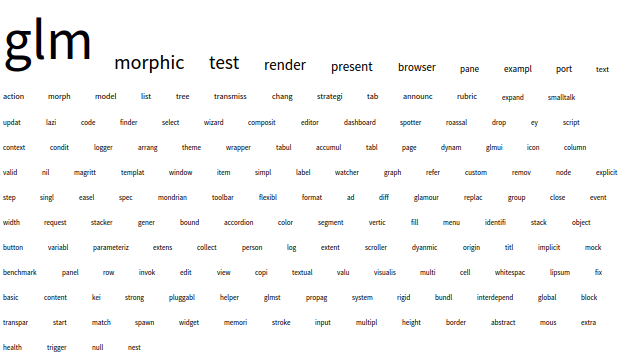
\includegraphics[width=\textwidth]{name_cloud}
\\
As we can see \textbf{GLM} is the suffix coming up the more often. Other suffix such as \textbf{test} \textbf{render} or \textbf{morphic} arise too. It seems that classes are named quite correcly in order to provide meta-information about their use.\\

We can perform the same analysis for methods or variable.Globally there is no bad smells coming up here. There is not randomly named classes variable or methods. Anyway, naming convention is quite a controversial issue, so we are not going deeper in the analysis here. 
\section{Metrics-based analysis}
 \subsection{Introduction}

\section{Conclusion}
\section{Annexes}

\end{document}
